\chapter{Grover's Search Algorithm}
\section{Introduction}
Searching an item in an unsorted table or array of size N costs a classical computer O(N) running time. Grover, in 1995 posited that a quantum computer can perform the same search in $O(\sqrt{N})$.Though this speedup is not as an exponential speedup as seen in prime factoring natural numbers (Shor's Algorithm), Grover's algorithm still has various applications such as speedup algorithms for NP-complete algorithms. In 1994, before Grover's algorithm, it was proved that a quantum computer needs to make atleast $\sqrt{N}$ queries to perform a successful search.


\section{Setup}
Let our sorted list contain $N=2^n$ elements. The length of the list is usually taken to be an exponential power of 2 for easier understanding as we can represent every element in the list by a state given by the superposition of the n qubits we'll be using. We define two function; An Oracle Function and a Diffusor Function that we will be repeatedly using in the algorithm.


\subsection{The Problem}
Let us model the problem as follows: Let f:\{1,2,3....N\} $\rightarrow$ \{0,1\} be a boolean function where it is given that f(a) = 1 for exactly one a $\epsilon$ \{1,......N\}. Obviously, a is the element we are looking for. Therefore, we can model the problem as finding the value of a such that f(a) = 1 .


\subsection{Qubits}
To start off, we prepare a uniform superposition of n qubits ($N = 2^n$; N is total number of elements.) Let $|\psi_t \rangle$ represent the state of the qubits at any iteration.
This can be easily done by using n hadamard gates $| s \rangle = H^{\otimes n} | 0 \rangle^n$ .
Therefore we get \[ |s \rangle = \frac{1}{\sqrt{N}} \sum_{x = 0}^{N -1} | x
\rangle. \].


\begin{figure}[!ht]
  \centering
  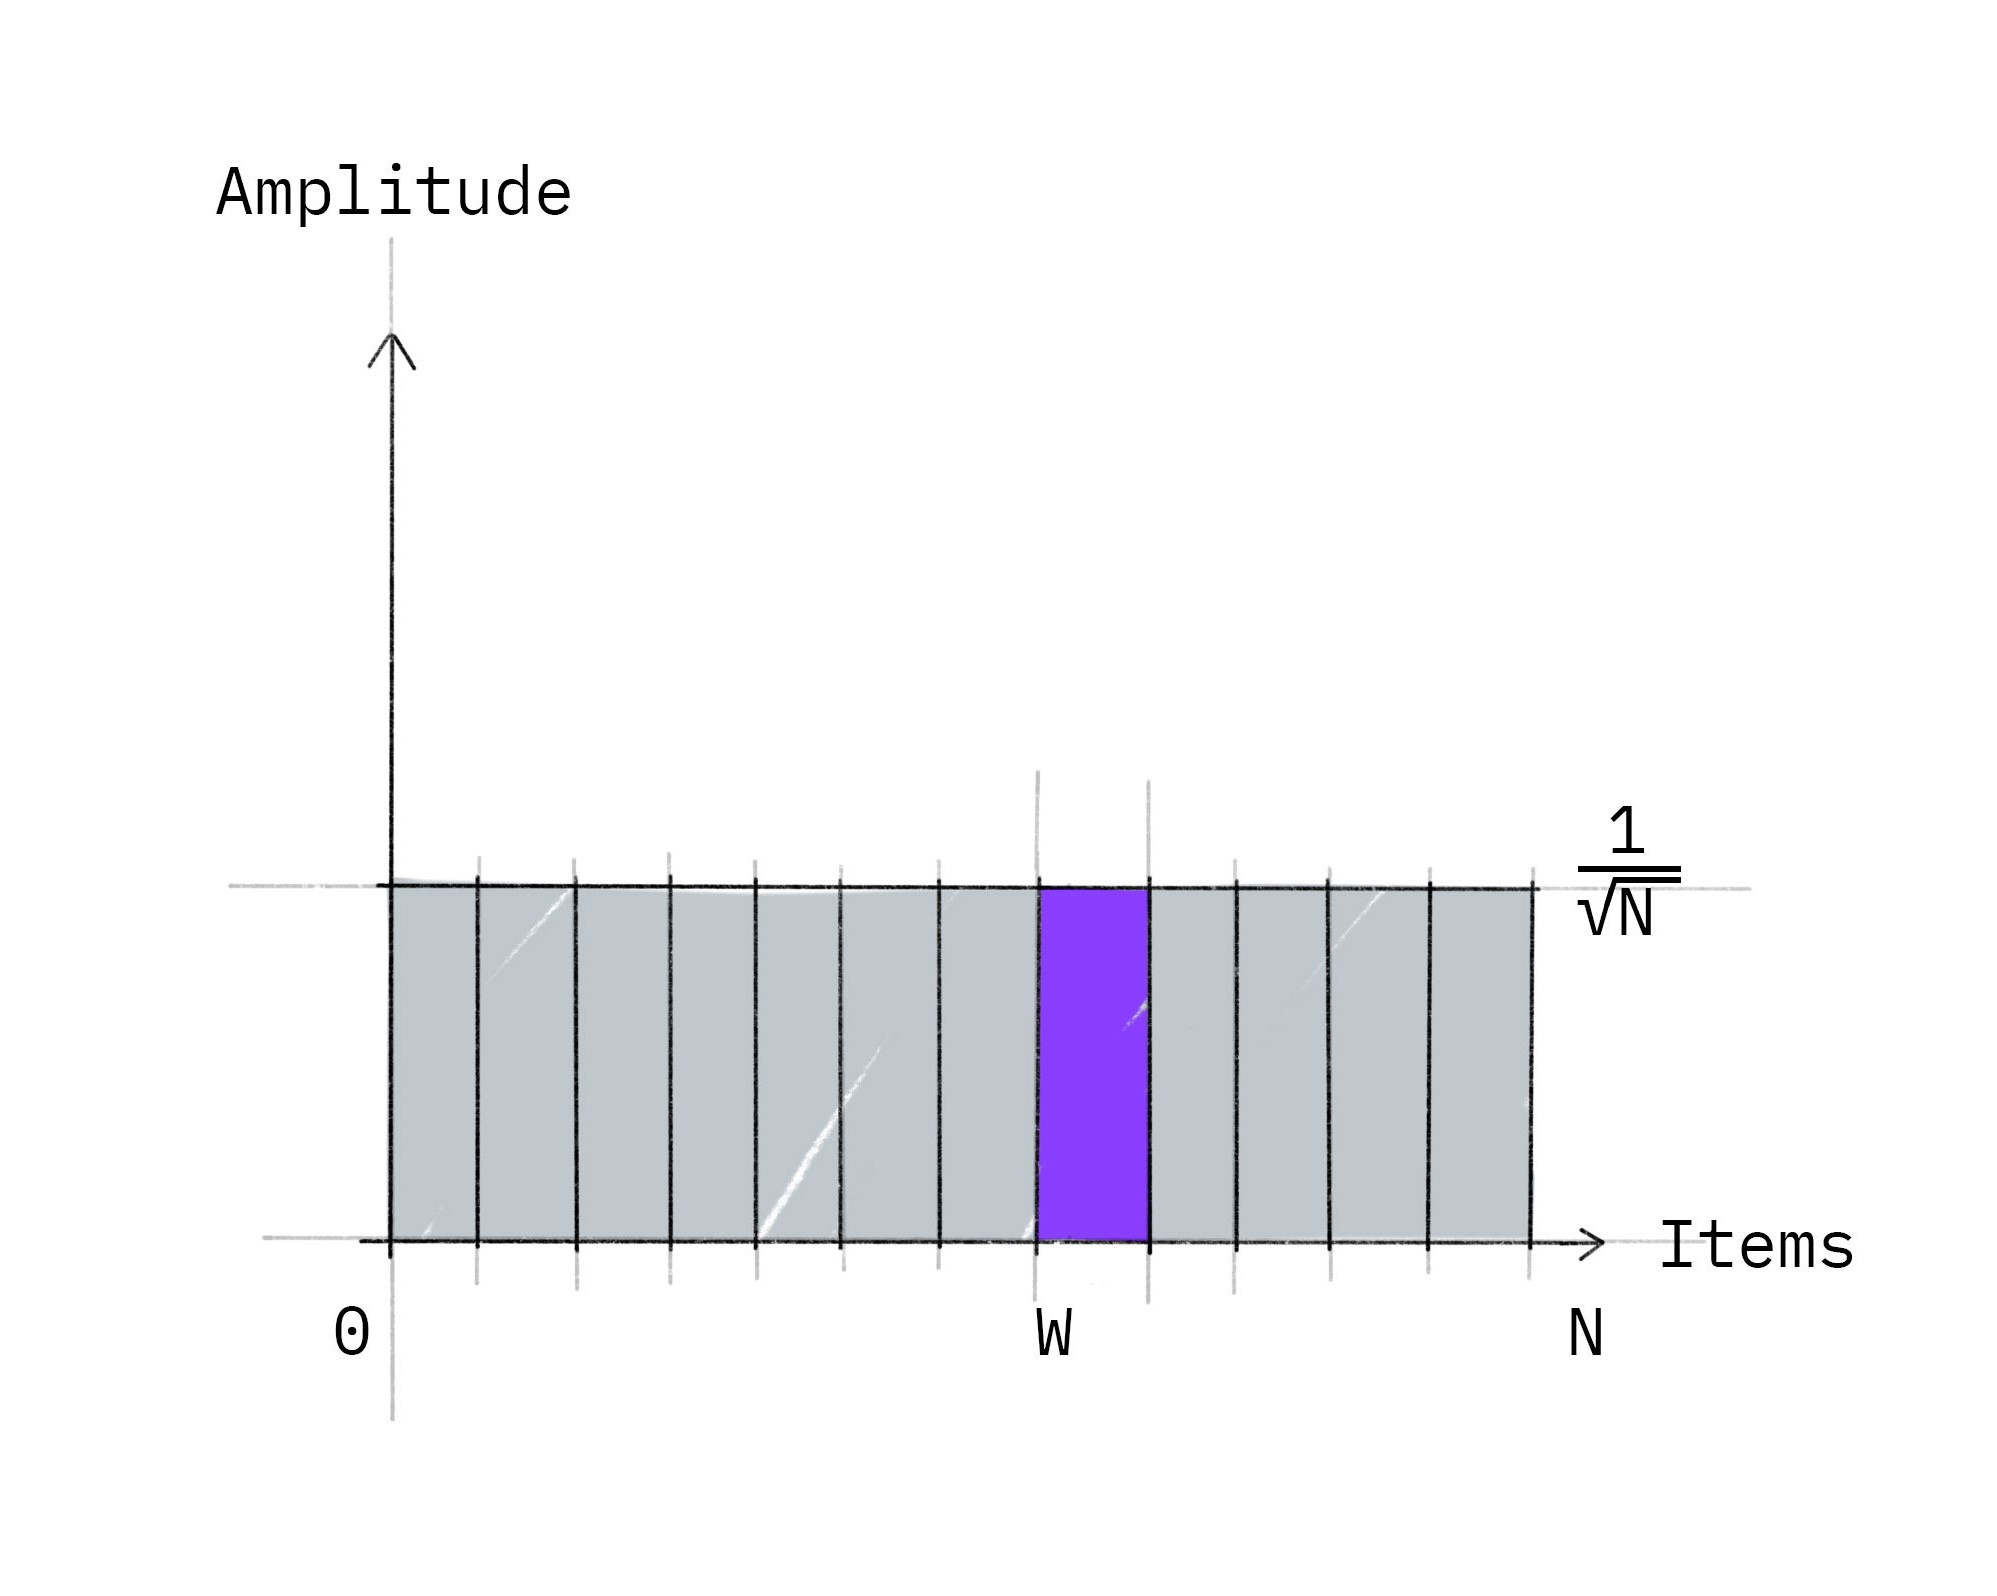
\includegraphics[width=5in]{grover_step1.jpg}
\end{figure}


\subsection{Oracle Function}
We define an oracle function for f:\{1,2,......N\} $\rightarrow$ \{0,1\} defined as: \\
\begin{align*}
 U_\omega|x\rangle =
    \begin{cases}
    |x\rangle \quad \text{if} \;  x \neq \omega \\
    -|x\rangle \quad \text{if} \; x = \omega
\end{cases}
\end{align*}

The oracle function will be a diagonal matrix, where the entry corresponding to the marked item will have a negative phase. Therefore our oracle function takes a proposed solution x, and returns f(x) = 0 if $x \neq \omega $ and f(x) = 1 for $x = \omega$ . Note that the oracle function depends on the answer we are searching for and changes accordingly with the answer we are looking for. The oracle  can be written as:
\[ U_\omega|x\rangle = (-1)^{f(x)}|x\rangle \] 

The oracle matrix will be a diagonal matrix defined as: \\ \\
\begin{center}
    
$ U_\omega = 
\begin{bmatrix}
(-1)^{f(0)} &   0         & \cdots &   0         \\
0           & (-1)^{f(1)} & \cdots &   0         \\
\vdots      &   0         & \ddots & \vdots      \\
0           &   0         & \cdots & (-1)^{f(2^n)} \\
\end{bmatrix} $ \end{center} 

Let $|a\rangle$ be the answer state.After creating a superposition of the qubits, 
 we now apply the oracle matrix to s. As explained in the setup before, the superposition obtained has the phase of the $|a\rangle$ flipped.
We have $ |\psi_t \rangle = (U_f)|s\rangle $.

\begin{figure}[!ht]
  \centering
  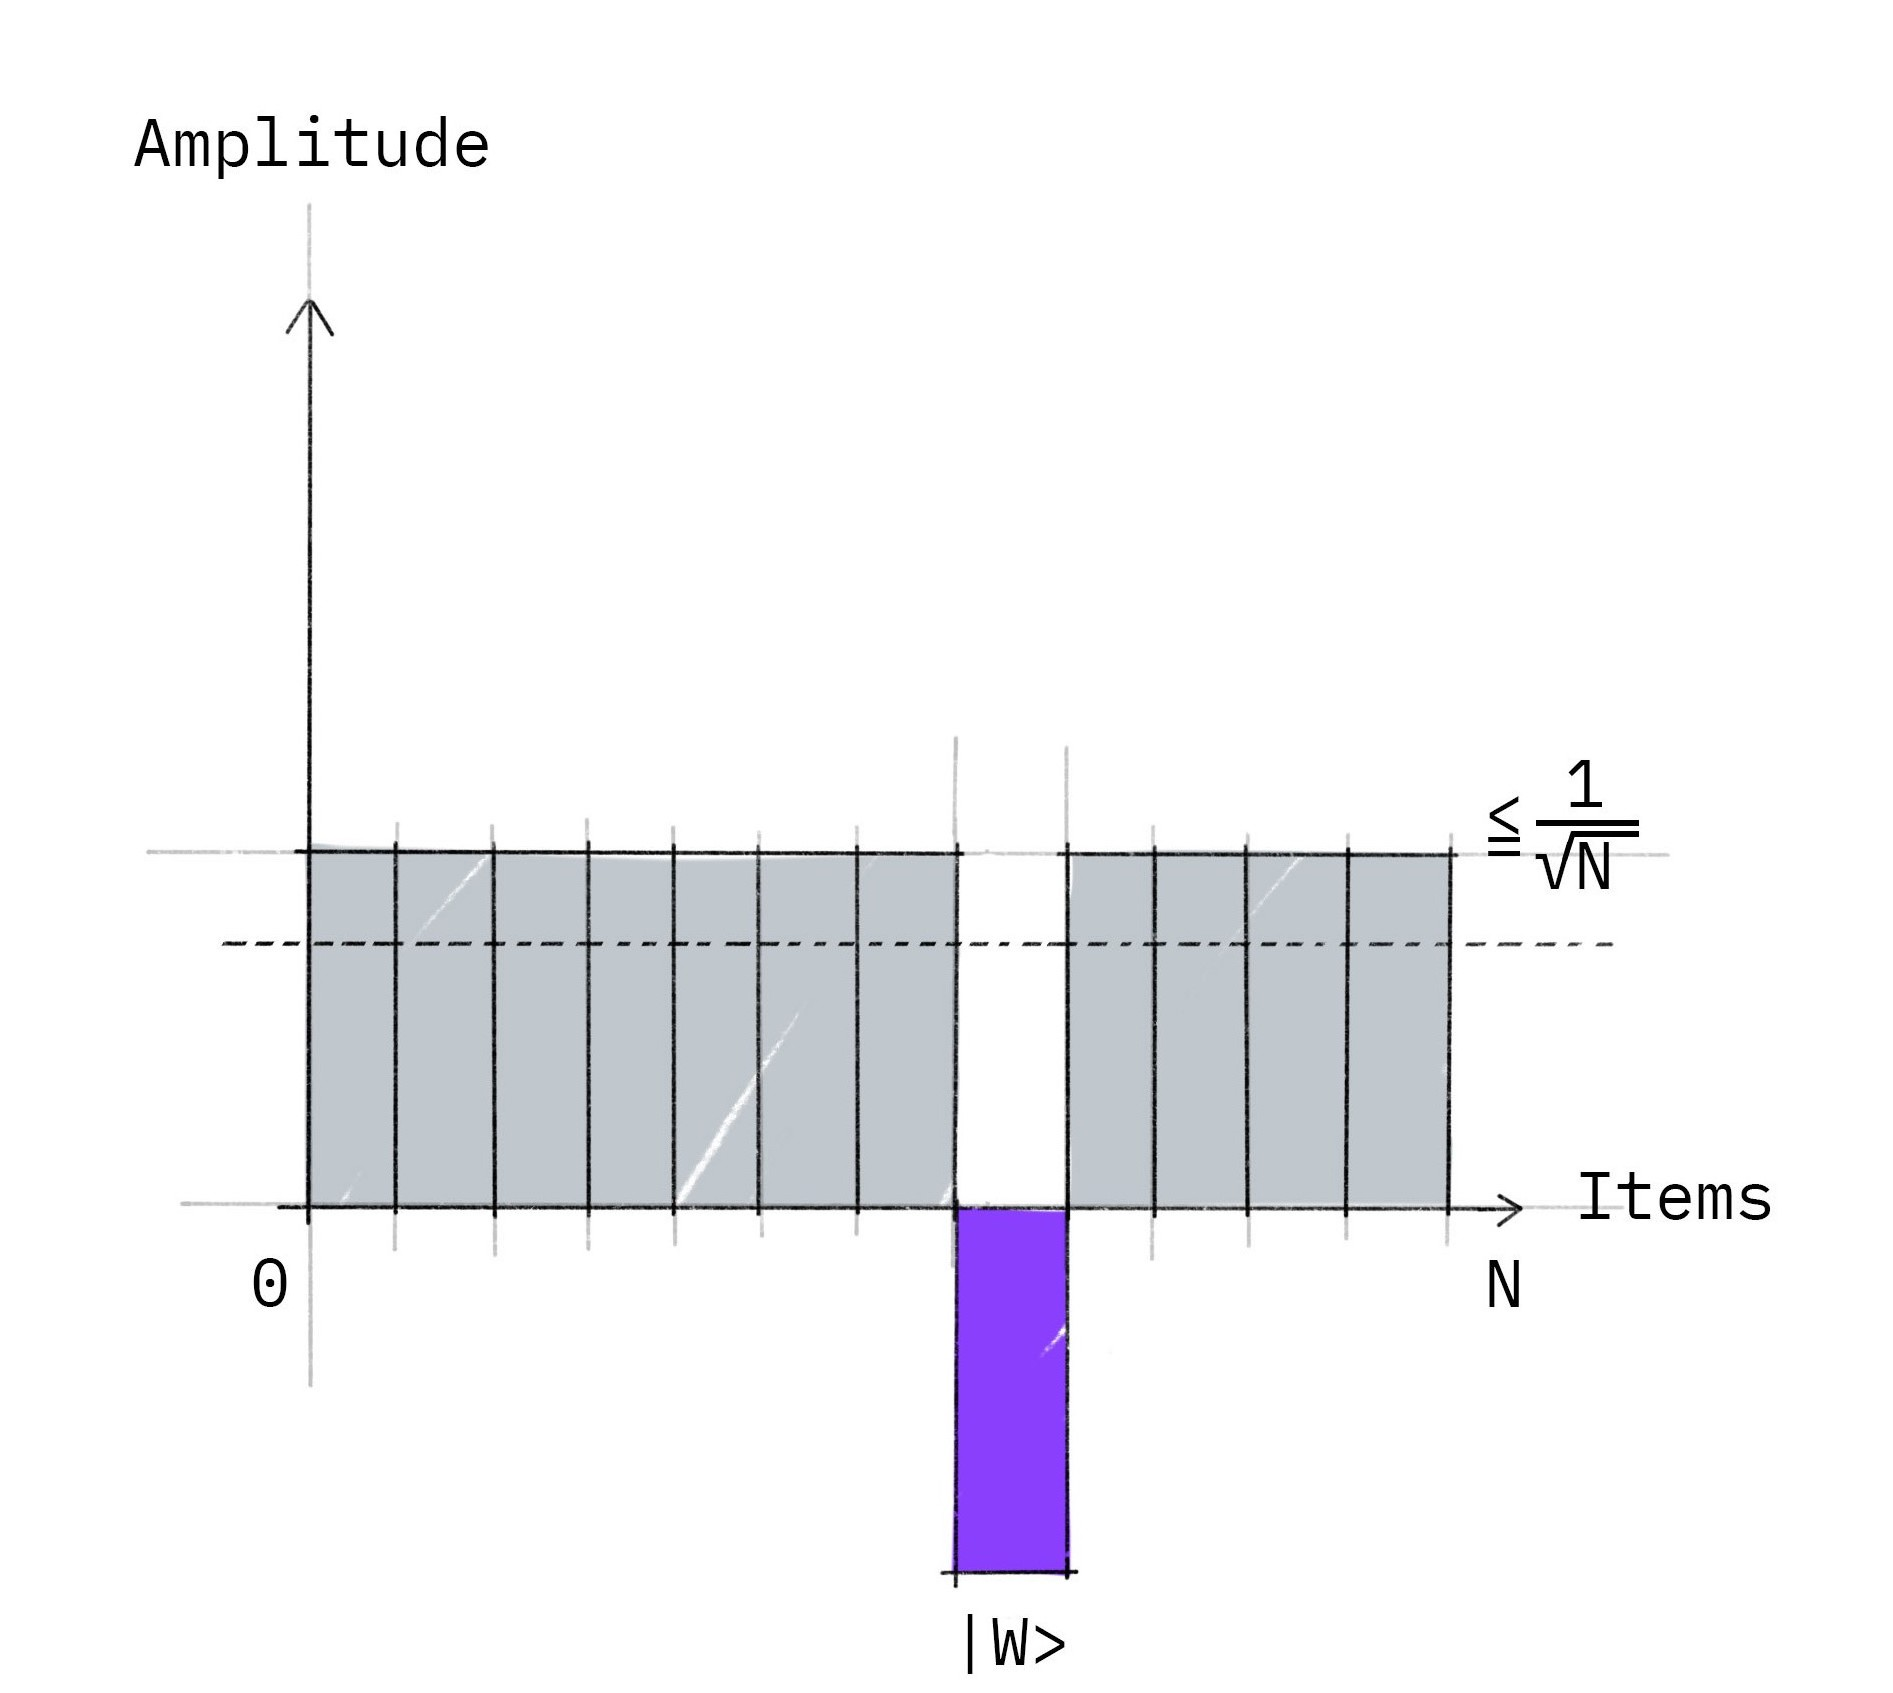
\includegraphics[scale = 0.15]{grover_step2.jpg}
\end{figure}


\subsection{Diffusor Function}
The Diffusor function, also known as the Grover Operator or the Amplitude Amplification Operator is a linear operator which takes as input n amplitudes and "flips them about their mean". It means taking a reflection of the amplitudes about their mean.
For example consider a superposition of 3 qubits with amplitudes : \\

\begin{align*}
    A( |x\rangle) = 
    \begin{cases}
    \frac{-1}{2\sqrt{2}} \quad \text{for} \; x = |011\rangle \\
    \frac{1}{2\sqrt{2}} \quad \text{otherwise}   
    \end{cases}
\end{align*}

 The two figures graphically show the amplitudes distribution before and after applying the Diffusion operator or flipping the amplitudes about its average.
 Mathematically the operator is defined as $U_s = 2|s\rangle \langle s| -1$.
 After applying the Diffusion Operator we get $|\psi_t \rangle = (U_s U_f) |s\rangle$.Now, one iteration of the algorithm is complete.
 

Now after one iteration(applying oracle and diffusion once)  we see that the amplitude of the answer state has increased. Ofcourse, our goal is to increase that amplitude as much as possible, (bring it close to 1) so that when we measure it, the qubit always collapses to the required answer state.

Initially, 
\[ A_0 = A_1 = ....A_{N-1} = 1/\sqrt{N} \]
 
Average of amplitudes after amplitude negation = $(1-2/N)1/\sqrt{N}$. After applying the diffusion operator, the ampltiude of the answer state which was $1/\sqrt{N}$ grows approximately by $1/\sqrt{N}$ every iteration. Therefore after t iterations, we get $|\psi_t\rangle = (U_s U_f)^t |s\rangle$
However, since we are dealing with amplitudes and not probabilities, the vector space's dimension enters as a square root. Therefore it is the amplitude, and not just the probability, that is being amplified in this procedure. 

% add the 3 images here. grover_step 1 to 3
\begin{figure}[!ht]
  \centering
  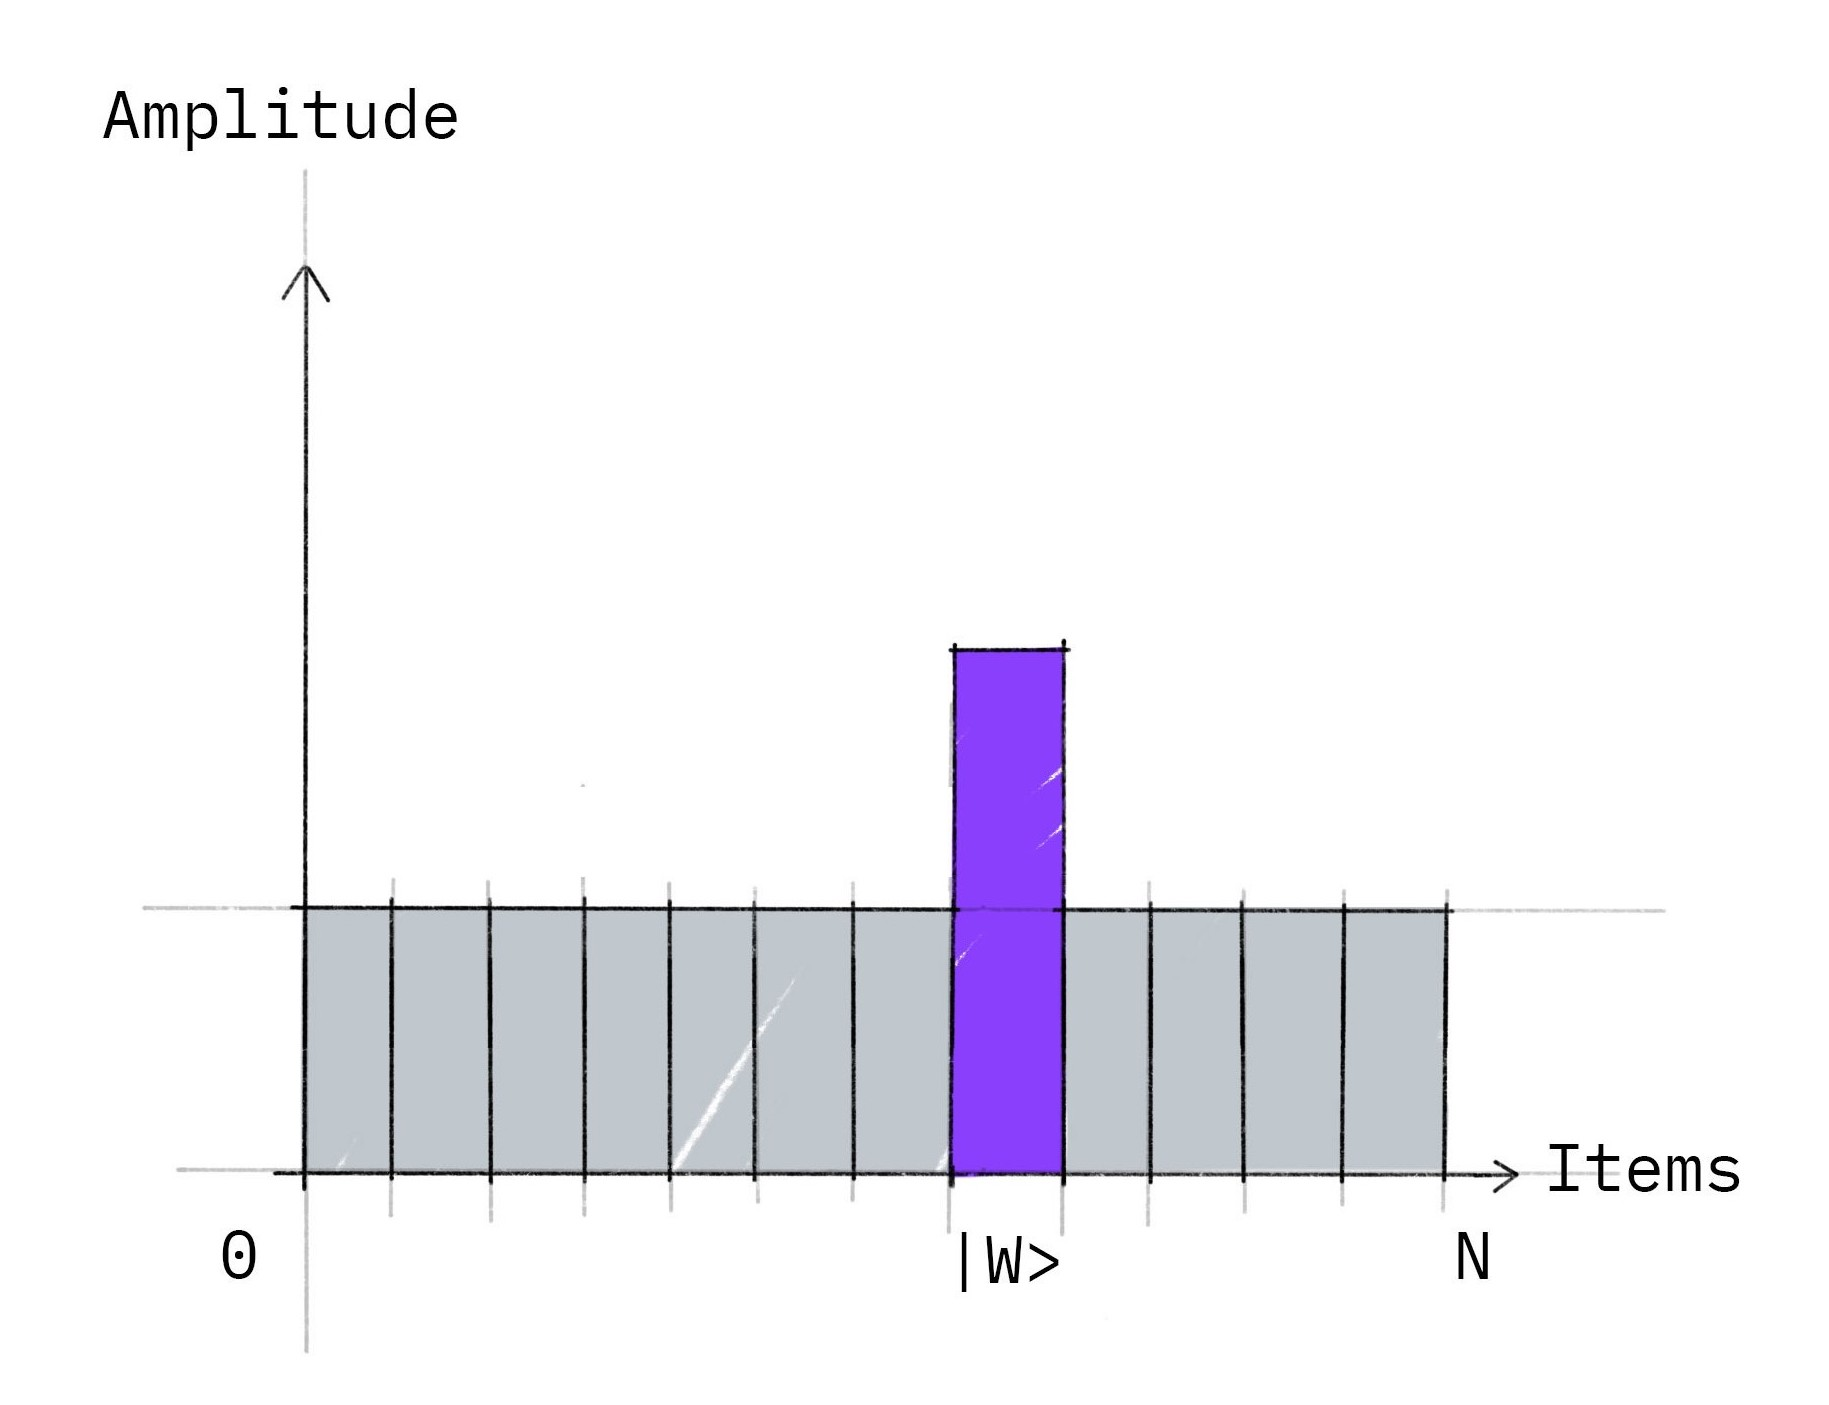
\includegraphics[scale = 0.15]{grover_step3.jpg}
\end{figure}


\section{Another Approach}
One approach of looking at the Grover's algorithm is to consider N different states and then after every iteration looking at the decrease in the amplitude of the non-answer states and the amplitude of the answer state trying to reach 1 in approximately $\sqrt{N}$ iterations.
The second approach stems from this idea that the non-answer states behave almost similarly and the superposition of the non-answer states be treated a single vector. Therefore we consider two states the answer state $|\omega\rangle$ and the superposition $|s\rangle$. These two vectors span a two dimensional- plane in the vector space $C^{N}$. These two vectors are not linearly independent or perpendicular as the vector $|\omega\rangle$ is a part of the superposition $|s\rangle$ with an amplitude $1/\sqrt{N}$. In the case that there are multiple solutions,  M , it can be shown that roughly \sqrt{N/M} iterations will suffice.



To resolve this problem, we introduce another vector $|s'\rangle$ which is obtained from removing the vector $|\omega\rangle$ from $|s\rangle$.

%add photo here for the superposition.
\begin{figure}[ht]
  \centering
  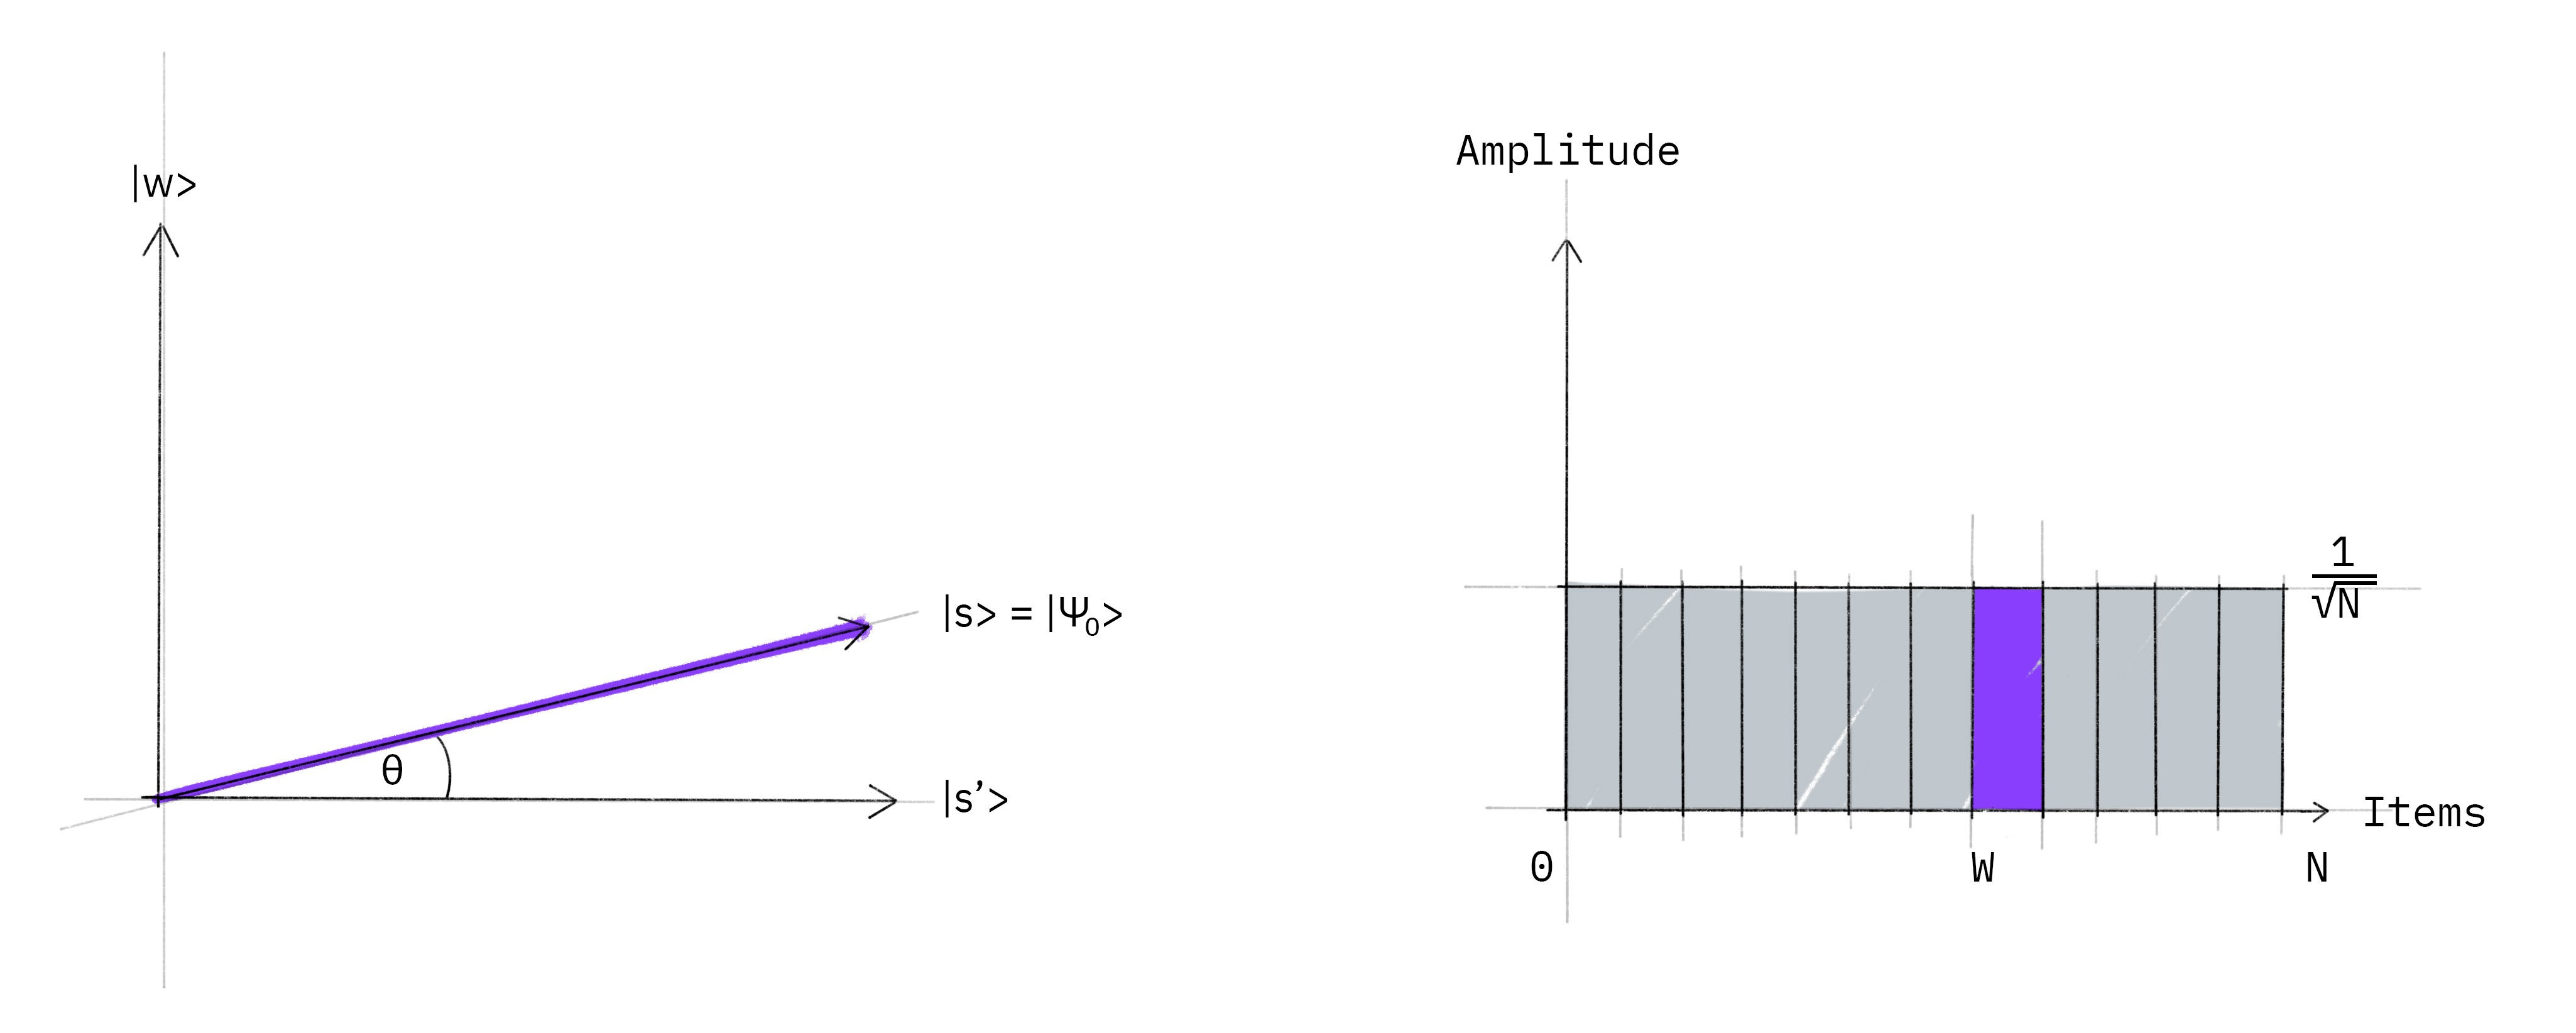
\includegraphics[scale = 0.09]{grover_step4.jpg}
\end{figure}


Now, the oracle function is supposed to invert the amplitude of the answer state $|\omega\rangle$, geometrically that transforms directly to taking a  reflection of the state $|s\rangle$ about the $|s'\rangle$ because this transformation means that the amplitude of $|\omega\rangle$ becomes negative resulting in amplitude negation

%add the photo here for grover_step5
\begin{figure}[h]
  \centering
  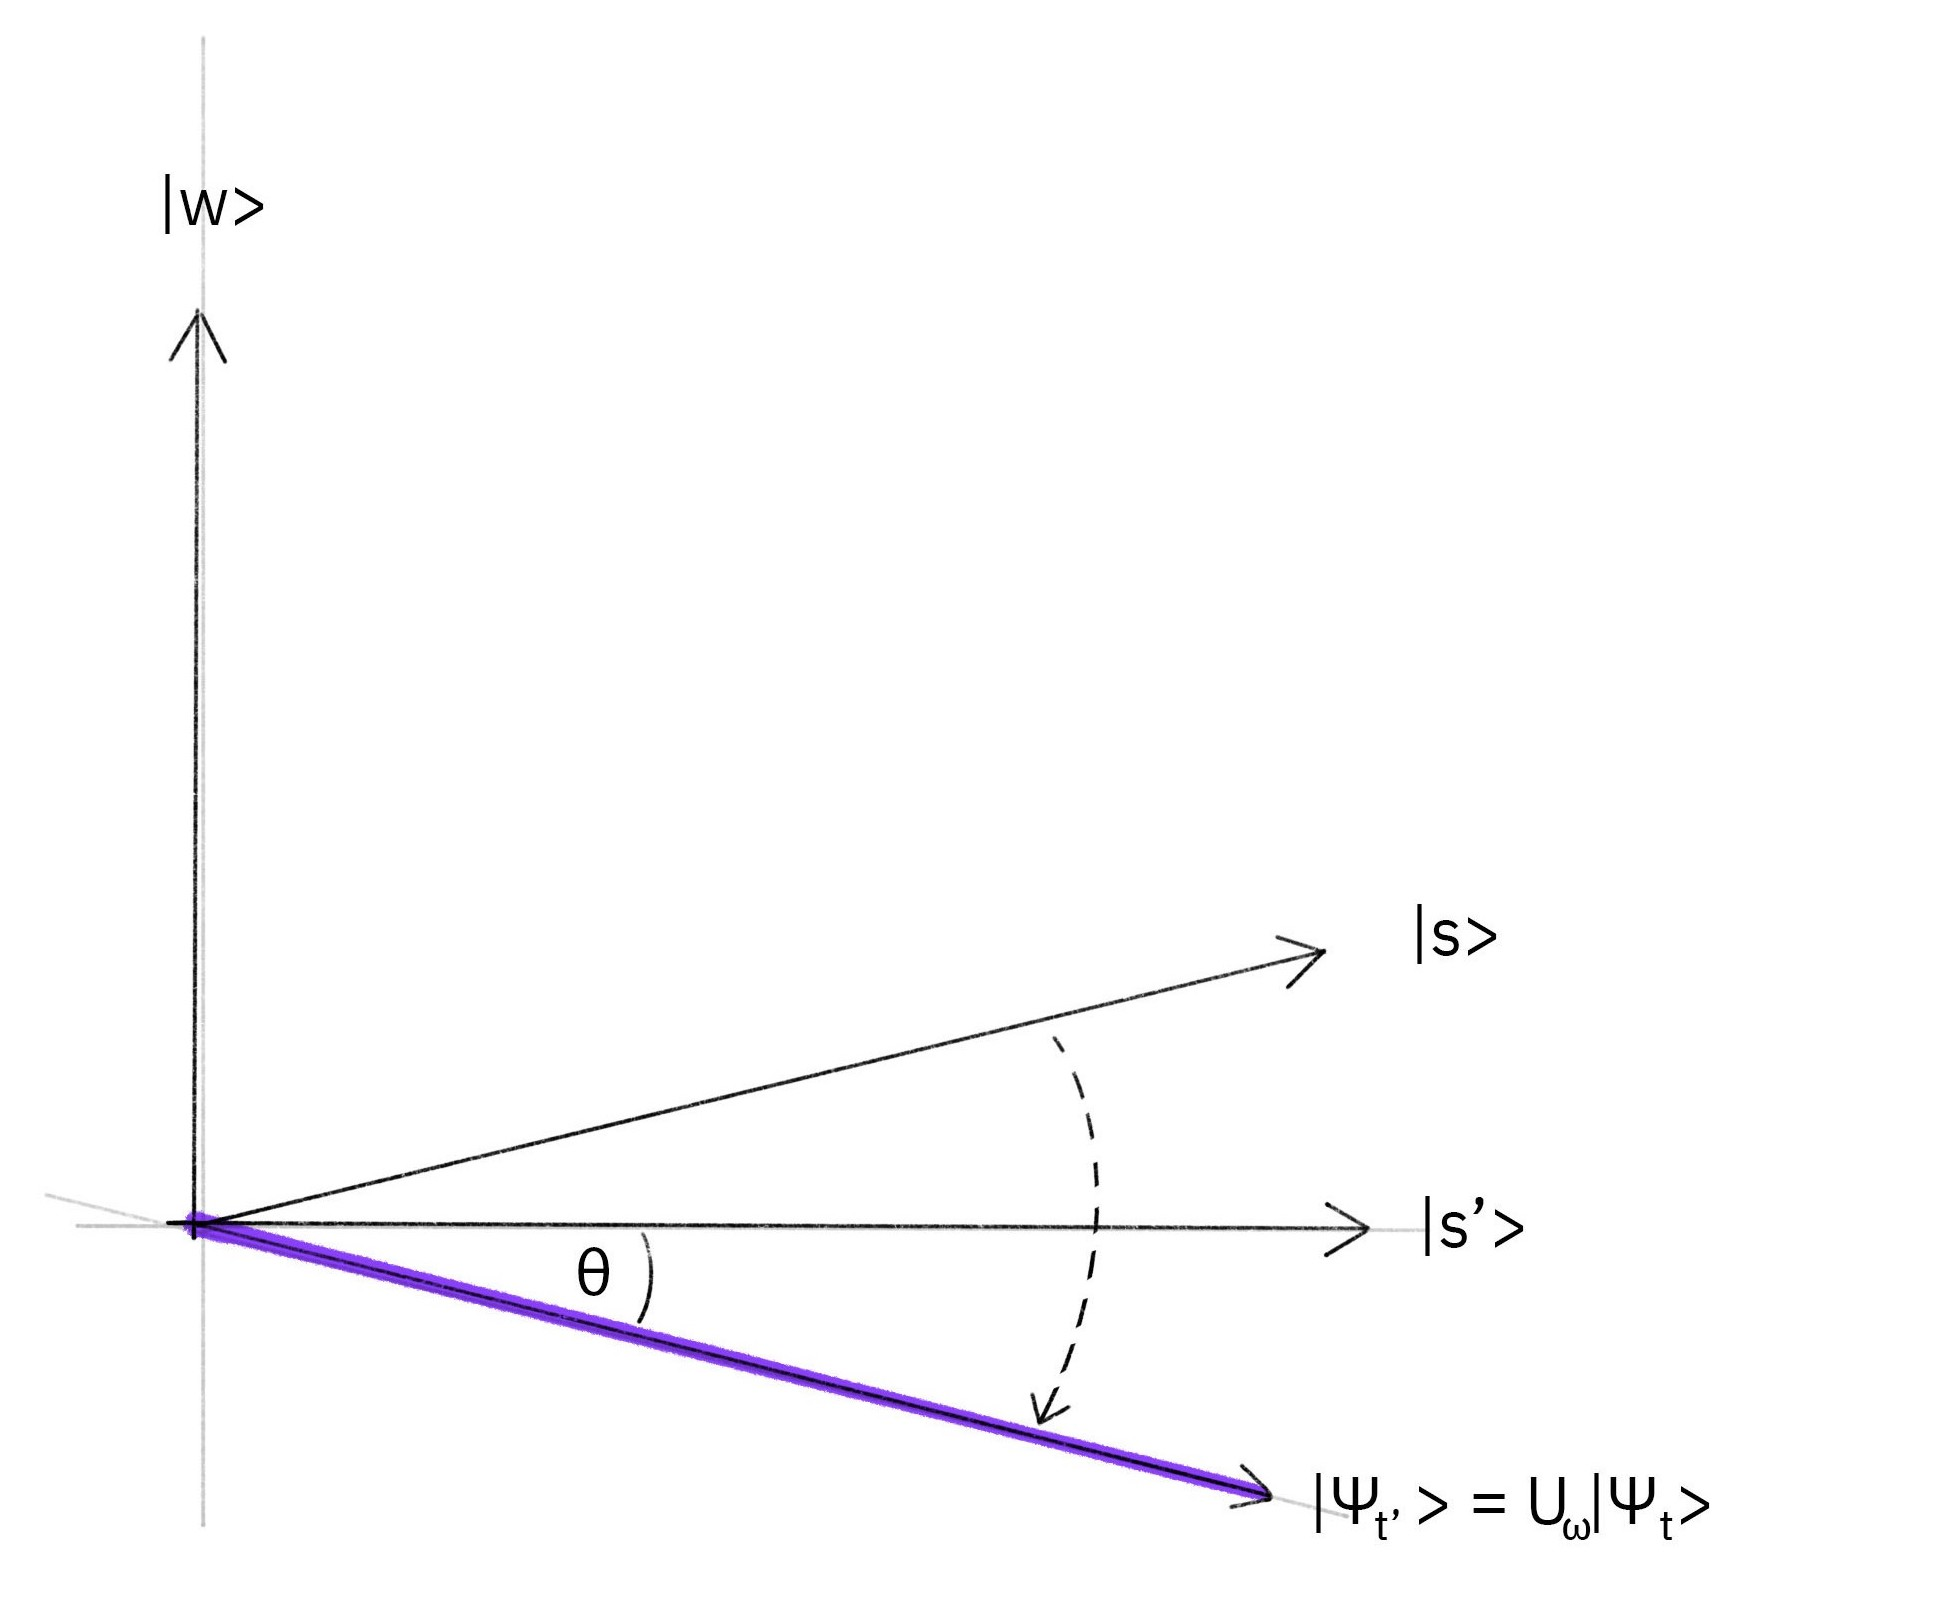
\includegraphics[scale = 0.1]{grover_step5.jpg}
\end{figure}

The Grover operator ($U_s$) takes the amplitudes and flips them about their mean which is equivalent to taking their reflection from $|s\rangle$ .The net effect of these two reflections, as we will see, is to increase the angle between the state and $|\omega\rangle$ and $|s\rangle$. Repeating this pair of reflections moves the
state farther and farther from $|s'\rangle$, and therefore closer and closer to $|\omega\rangle$. Once it is close enough,measuring the state results in outcome a with good probability.
% add photo grover_step6
\begin{figure}[h]
  \centering
  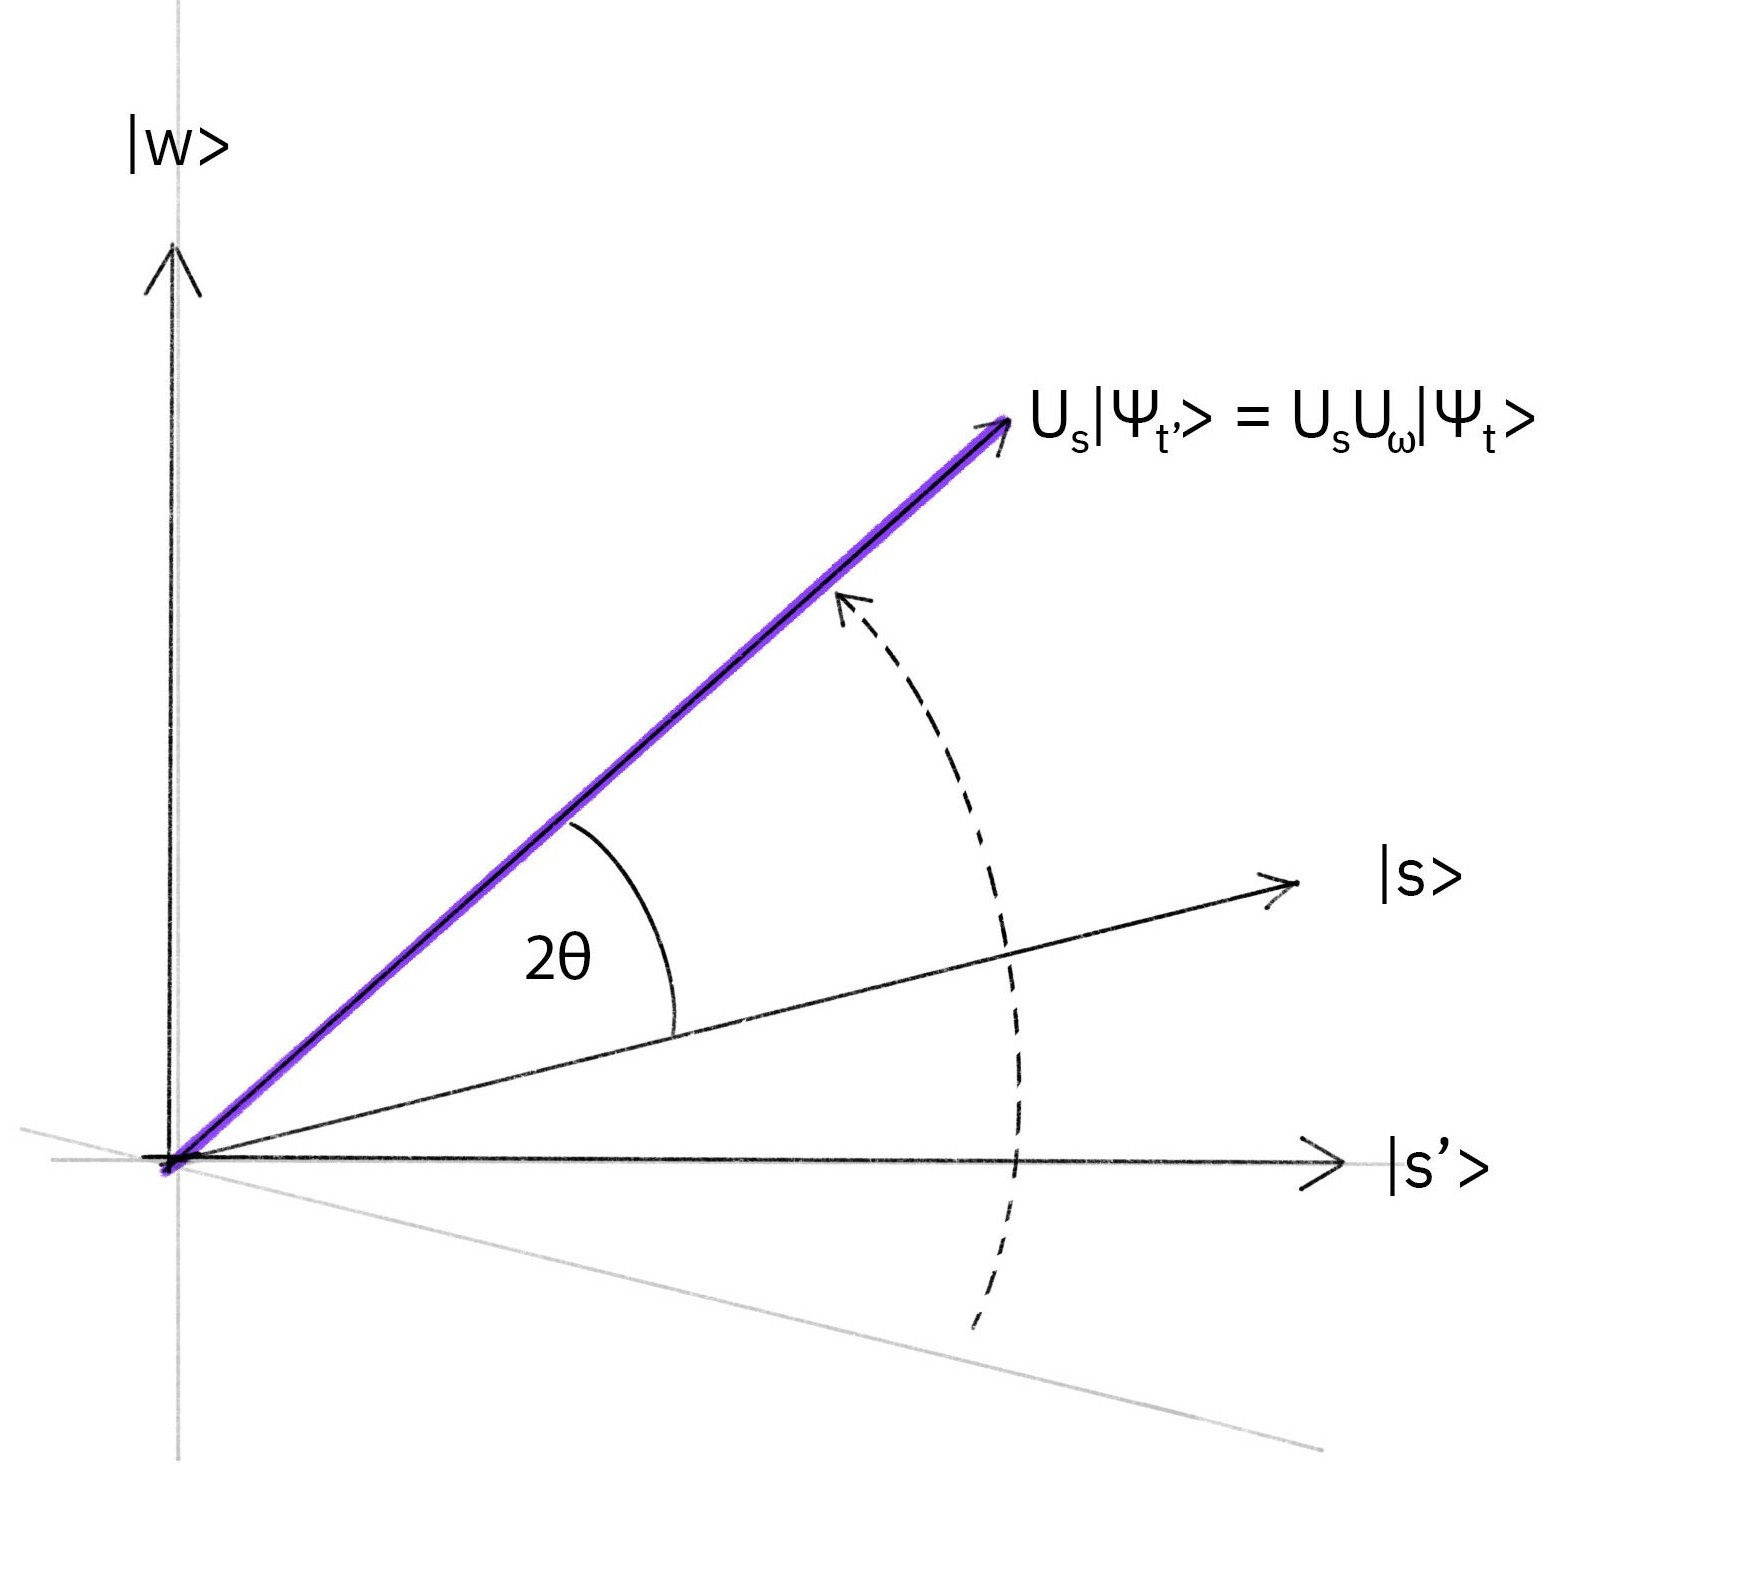
\includegraphics[scale = 0.1]{grover_step6.jpg}
\end{figure}
\pagebreak
\section{More about the quantum oracle}
From our boolean function f:\{1,2,3....N\} $\rightarrow$ \{0,1\} we know that we can construct a quantum circuit $U_f$ to carry out this computation. Since we know f can be computed classically in polynomial time, we can
also compute it in superposition: \bigskip
\[ \sum_x\alpha_x|x\rangle|0\rangle \rightarrow \sum_x\alpha_x |x\rangle |f(x)\rangle \]

There is also a tricky way to put our result into a form that equally contains all of the information
relevant to our problem. We can put the answer register in the superposition $\ket{-}$, so that when we
implement f the information is stored in the phase or sign of the result:

In more detail: 
    % put the equation here.
\begin{aligned} U_f:\; \sum_{x} \alpha_{x}
  |x\rangle \left(\frac{|0\rangle - |1\rangle}{\sqrt{2}} \right) & \mapsto
  \sum_{x} \alpha_{x} \left(\frac{ |x\rangle |f(x)\rangle - |x\rangle
  |\overline{f(x)}\rangle}{\sqrt{2}} \right) \\ & = \sum_{x} \alpha_{x}
  |x\rangle \left(\frac{|f(x)\rangle - |\overline{f(x)}\rangle}{\sqrt{2}}
  \right) \\ & = \sum_{x} \alpha_{x} |x\rangle (-1)^{f(x)}
  \left(\frac{|0\rangle - |1\rangle}{\sqrt{2}}\right)\end{aligned}

$U_f$ has the property that when x = a, the phase of the state will be multiplied by -1. We will see that this implementation of the circuit is equivalent to a reflection over the vector $|s'\rangle$

\section{Quantum Circuit}
We now go through the example of Grover's algorithm for 3 qubits with two marked states  |101⟩  and  |110⟩ , following the implementation found in Reference [2]. The quantum circuit to solve the problem using a phase oracle is:
\begin{figure}[!ht]
  \centering
  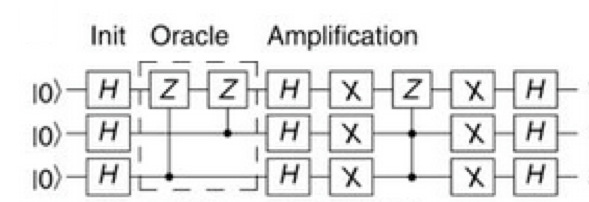
\includegraphics[width=3in]{grover_circuit_3qubits.png}
\end{figure}

\section{Analysis and Comparison}
As compared to our normal linear search on a shuffled random list, Grover's search gives us a quadratic speed-up where a classical search takes O(N) times, Grover's search runs in O($\sqrt{N}$) of time. However, this a probabilistic model where in we consciously try to increase the amplitude of the answer state which can be increased to approximately 1 in about $\sqrt{N}$ iterations but there may be a small probability that we may not find the answer in these iterations.
